\begin{figure}
\centering	
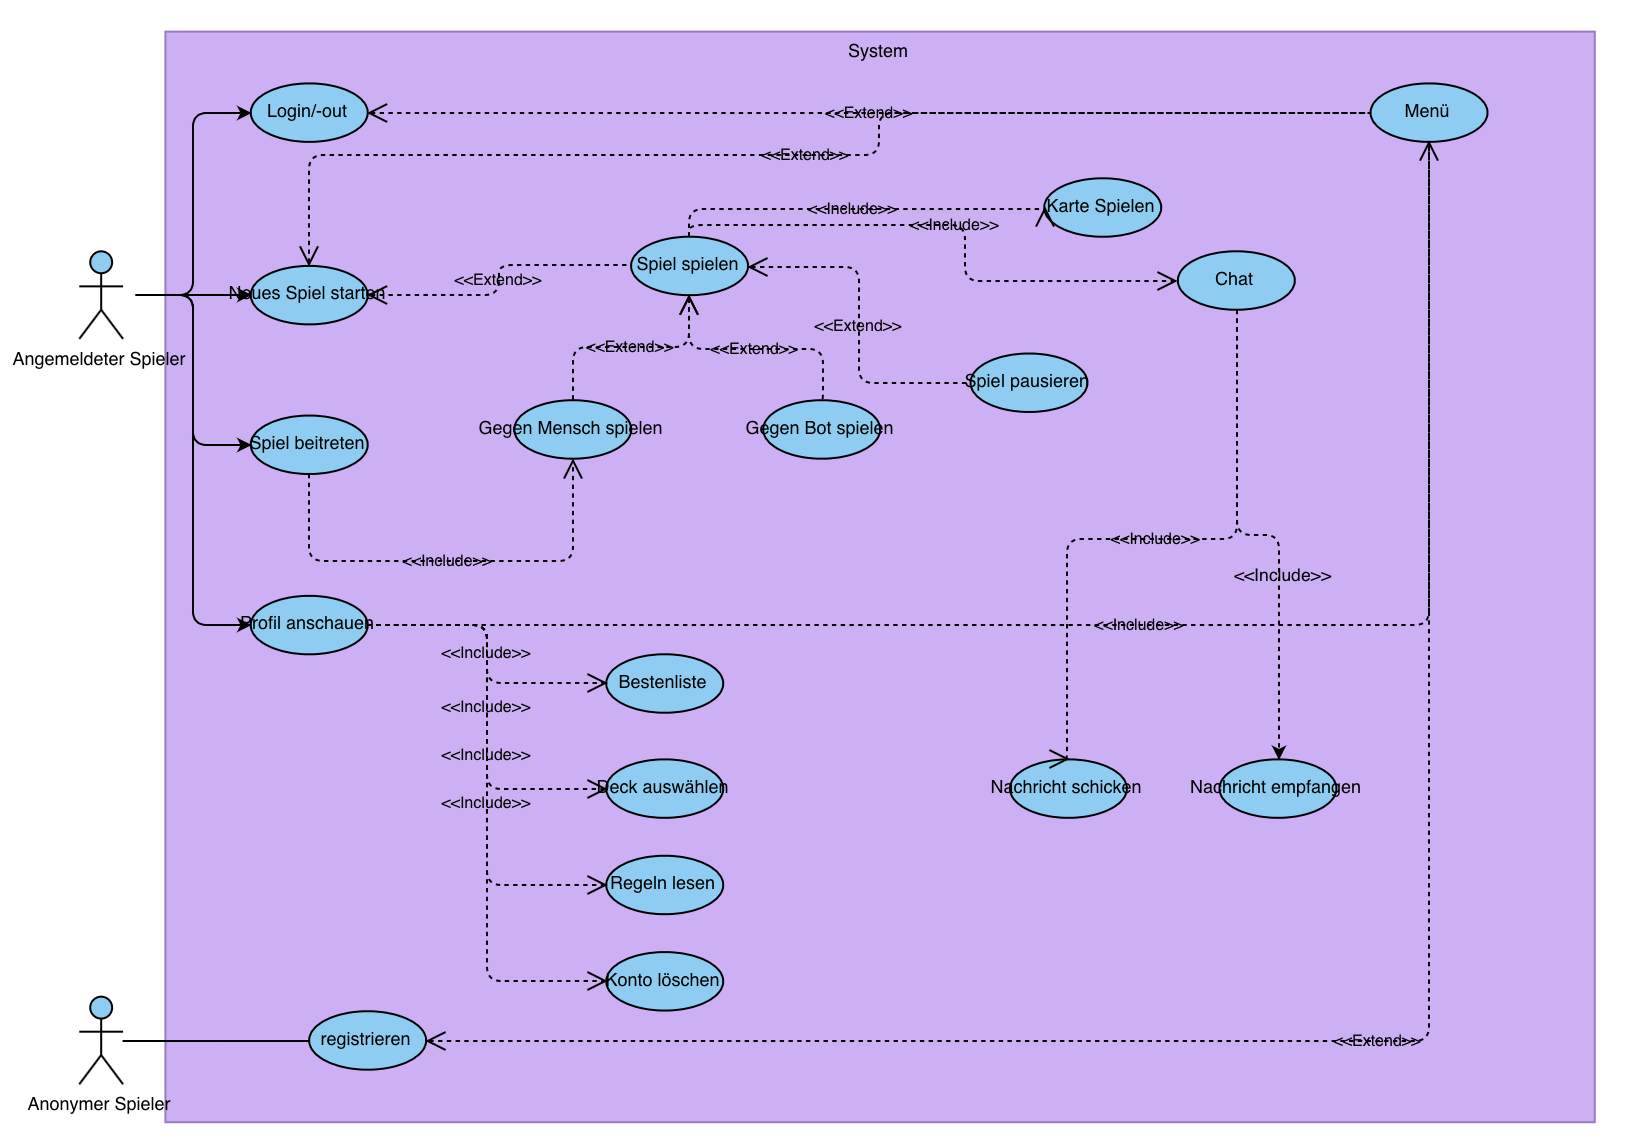
\includegraphics[width=0.9\textwidth]{img/UCD.jpg}
\label{fig:sys}
\caption{Beispiel für ein Systemgrenzediagramm (Use Case Diagramm), das vor Abgabe anzupassen ist.}
\end{figure}

\section{Systemgrenze (Use Case Diagramm)}

Die Systemgrenze wird in der Abbildung~\ref{fig:sys} dargestellt\footnote{Weitere Erklärungen und Spezifizierungen, die sich auf Abgrenzungen der Verantwortlichkeiten vom System und weiteren Akteuren/Systemen beziehen, können hier spezifiziert werden.}. 


\section{Beschreibungen der Anwendungsfälle}

\newcounter{uc}\setcounter{uc}{10}

\begin{description}[leftmargin=5em, style=sameline]

	\begin{lhp}{uc}{UC}{uc:register}
		\item [Name:] Registrieren
		\item [Ziel:] Ein neuer Spieler kann sich registrieren um ein Profil zu erhalten.
		\item [Akteure:] Anonymer Spieler
		\item [Vorbedingungen:] Spiel is gestartet und befindet sich im Startbildschirm.
		\item [Eingabedaten:] Zugriffsdaten~\ref{daten:benutzername}~\ref{daten:passwort}.
		\item [Beschreibung:] \hfill\\
				1. Der Spieler wählt den Punkt Registrieren aus.\\
				2. Das System zeigt das Registrierungsformular an.\\
				3. Der Spieler sendet das Formular mit Name und Passwort ab.\\
				4. Das System speichert die Daten und zeigt wieder das Hauptmenu an.\\
		\item [Ausnahmen:] Bei Beendigung wird nichts gespeichert. Das System bleibt in seinem aktuellen Zustand.
		\item [Ergebnisse und Outputdaten:] Das Profil ist in der Datenbank. Der \textbf{Anonyme Spieler} wird zum \textbf{Spieler}
		\item [Systemfunktionen] \ref{funk:zugriff} \ref{funk:start}
	\end{lhp}

	\begin{lhp}{uc}{UC}{uc:login}
		\item [Name:] Anmelden
		\item [Ziel:] Ein Spieler kann sich anmelden um im Spiel sein persönliches Profil zu verwenden.
		\item [Akteure:] Spieler
		\item [Vorbedingungen:] Spiel is gestartet und befindet sich im Startbildschirm.
		\item [Eingabedaten:] Zugriffsdaten~\ref{daten:benutzername}~\ref{daten:passwort}.
		\item [Beschreibung:] \hfill\\
				1. Der Spieler wählt den Punkt Anmelden aus.\\
				2. Das System zeigt das Anmeldeformular an.\\
				3. Der Spieler sendet das Formular mit Name und Passwort ab.\\
				4. Das System prüft die Richtigkeit vom Passwort und wechselt gegebenenfalls auf das Profil des Nutzers. Danach wird das Hauptmenu angezeigt.\\
		\item [Ausnahmen:] Ist das Passwort falsch, wird eine Fehlermeldung angezeigt. In 4. wird das Hauptmenu nicht betretten.
		\item [Ergebnisse und Outputdaten:] Das aktive Profil wurde geändert. Der \textbf{Spieler} ist nun eingeloggt und kann spielen.
		\item [Systemfunktionen] \ref{funk:zugriff} \ref{funk:start}
	\end{lhp}

	\begin{lhp}{uc}{UC}{uc:logout}
		\item [Name:] Abmelden
		\item [Ziel:] Ein Spieler kann sich abmelden.
		\item [Akteure:] Spieler
		\item [Vorbedingungen:] Spieler ist angemeldet. Spieler ist im Hauptmenu.
		\item [Eingabedaten:] Zugriffsdaten~\ref{daten:benutzername}~\ref{daten:passwort}.
		\item [Beschreibung:] \hfill\\
				1. Der Spieler wählt den Menupunkt Abmelden aus.\\
				2. Das System meldet den Nutzer ab, danach wird der Startbildschirm angezeigt.\\
		\item [Ausnahmen:] Keine
		\item [Ergebnisse und Outputdaten:] Das aktive Profil wurde geändert. Der \textbf{Spieler} ist nun eingeloggt.
		\item [Systemfunktionen] \ref{funk:zugriff} \ref{funk:menu}
	\end{lhp}

	\begin{lhp}{uc}{UC}{uc:delete}
		\item [Name:] Konto löschen
		\item [Ziel:] Spieler entfernt seine Daten aus dem System.
		\item [Akteure:] Spieler
		\item [Vorbedingungen] Spieler ist im Hauptmenu.
		\item [Eingabedaten:] Keine
		\item [Beschreibung:] \hfill\\
				1. Der Spieler wählt Menupunkt Einstellungen aus.\\
				2. Das System zeigt das Eintsellungsfenster.\\
				3. Der Spieler wählt den Punkt Profil löschen aus.\\
				4. Das System entfernt alle Daten des Spielers aus der Datenbank und zeigt den Startbildschirm an.
		\item [Ausnahmen:] Keine
		\item [Ergebnisse und Outputdaten:] Der \textbf{Spieler} wird zum \textbf{anonymen Spieler}.
		\item [Systemfunktionen:] \ref{funk:zugriff} \ref{funk:menu}
	\end{lhp}

	\begin{lhp}{uc}{UC}{uc:change}
		\item [Name:] Passwort ändern.
		\item [Ziel:] Spieler ändert sein Passwort.
		\item [Akteure:] Spieler
		\item [Vorbedingungen] Spieler ist angemeldet. Spieler ist im Hauptmenu.
		\item [Eingabedaten:] altes Passwort und neues Passwort \ref{daten:passwort}
		\item [Beschreibung:] \hfill\\
				1. Der Spieler wählt Menupunkt Profil aus.\\
				2. Das System zeigt das Profil.\\
				3. Der Spieler wählt den Punkt Passwort ändern aus.\\
				4. Das System zeigt das Änderungsformular.\\
				5. Der Spieler sendet das Formular mit altem und neuem Passwort ab.\\
				6. Das System prüft die Richtigkeit des Passworts und ändert gegebenenfalls die Daten des Spielers in der Datenbank.
		\item [Ausnahmen:] Ist das Passwort falsch, wird eine Fehlermeldung angezeigt. In 6. wird das Passwort nicht geändert.
		\item [Ergebnisse und Outputdaten:] Das Passwort ist geändert.
		\item [Systemfunktionen:] \ref{funk:zugriff} \ref{funk:menu}
	\end{lhp}
	
	\begin{lhp}{uc}{UC}{uc:profil}
		\item [Name:] Profil ansehen
		\item [Ziel:] Spieler schaut sich sein Profil an.
		\item [Akteure:] Spieler
		\item [Vorbedingungen] Spieler ist angemeldet. Spieler ist im Hauptmenu.
		\item [Eingabedaten:] Keine
		\item [Beschreibung:] \hfill\\
			1. Der Spieler wählt den Menupunkt Profil.\\
			2. Das System zeigt das Profil und alle Daten an.\\
			3. Der Spieler schaut sich seine Bestenliste an.
		\item [Ausnahmen:] Beim Verlassen landet der Spieler im Hauptmenu.
		\item [Ergebnisse und Outputdaten:] Spieler ist in seinem Profil.
		\item [Systemfunktionen:] \ref{funk:profil} \ref{funk:menu} \ref{funk:bestenliste}
	\end{lhp}

	\begin{lhp}{uc}{UC}{uc:regeln}
		\item [Name:] Regeln lesen
		\item [Ziel:] Spieler kann Regeln nachlesen.
		\item [Akteure:] Spieler
		\item [Vorbedingungen] Spieler ist im Hauptmenu.
		\item [Eingabedaten:] Keine
		\item [Beschreibung:] \hfill\\
				1. Der Spieler wählt Menupunkt Regeln aus.\\
				2. Das System zeigt die Regeln an.
		\item [Ausnahmen:] Beim Verlassen landet der Spieler im Hauptmenu.
		\item [Ergebnisse und Outputdaten:] Regeln werden angezeigt.
		\item [Systemfunktionen:] \ref{funk:menu}
	\end{lhp}

	\begin{lhp}{uc}{UC}{uc:comp}
		\item [Name:] Spiel gegen Computer.
		\item [Ziel:] Spieler startet Spiel gegen Computer.
		\item [Akteure:] Spieler
		\item [Vorbedingungen] Spieler ist im Hauptmenu.
		\item [Eingabedaten:] Keine
		\item [Beschreibung:] \hfill\\
				1. Der Spieler wählt den Menupunkt Spiel gegen Computer aus.\\
				2. Das System startet ein Spiel gegen Computer und zeigt das Spielfeld an.
		\item [Ausnahmen:] Beim Verlassen landet der Spieler im Hauptmenu.
		\item [Ergebnisse und Outputdaten:] Spieler befindet sich im Spiel. Spieler ist am Zug.
		\item [Systemfunktionen:] \ref{funk:spielverw} \ref{funk:bots}
	\end{lhp}

	\begin{lhp}{uc}{UC}{uc:erstellen}
		\item [Name:] Spielraum erstellen.
		\item [Ziel:] Spieler erstellt einen Spielraum für das Spiel mit Freunden.
		\item [Akteure:] Spieler
		\item [Vorbedingungen] Spieler ist im Hauptmenu.
		\item [Eingabedaten:] Keine
		\item [Beschreibung:] \hfill\\
				1. Der Spieler wählt den Menupunkt Spiel gegen Freunde aus.\\
				2. Das System fragt ob ein Spielraum erstellt oder beigetretten werden soll.\\
				3. Der Spieler wählt Menupunkt Spielraum erstellen.\\
				4. Das System erstellt einen Spielraum, den der Spieler leitet.
		\item [Ausnahmen:] Bei Beendigung oder Verbindungsfehler landet der Spieler im Hauptmenu und der Spielraum wird gelöscht.
		\item [Ergebnisse und Outputdaten:] Spieler befindet sich im Spielraum. Weiter Spieler können den Raum betretten.
		\item [Systemfunktionen:] \ref{funk:spielraum} \ref{funk:menu}
	\end{lhp}

	\begin{lhp}{uc}{UC}{uc:beitreten}
		\item [Name:] Spielraum beitretten.
		\item [Ziel:] Spieler tritt dem Spielraum eines anderen Spielers bei.
		\item [Akteure:] Spieler1, Spieler2, weitere Spieler
		\item [Vorbedingungen] Spieler1 ist Leiter eines Spielraums. Spieler2 ist im Hauptmenu. optional: weiter Spieler sind im Spielraum.
		\item [Eingabedaten:] Keine
		\item [Beschreibung:] \hfill\\
				1. Spieler2 wählt den Menupunkt Spiel gegen Freunde aus.\\
				2. Das System fragt ob ein Spielraum erstellt oder beigetretten werden soll. \\
				3. Spieler2 wählt Menupunkt Spielraum beitretten \\
				4. Das System fügt Spieler2 zum Spielraum hinzu und teilt Spieler1 mit, dass Spieler2 beigetretten ist.
		\item [Ausnahmen:] Bei Beendigung oder Verbindungsfehler landet Spieler2 im Hauptmenu.
		\item [Ergebnisse und Outputdaten:] Alle Spieler befinden sich im Spielraum
		\item [Systemfunktionen:] \ref{funk:spielraum} \ref{funk:menu}
	\end{lhp}

	\begin{lhp}{uc}{UC}{uc:spielraumdelete}
		\item [Name:] Spielraum löschen.
		\item [Ziel:] Spielraumleiter löscht den Spielraum.
		\item [Akteure:] Spieler1 und weitere Spieler
		\item [Vorbedingungen] Spieler1 ist Leiter eines Spielraums. Alle anderen Spieler sind im Spielraum von Spieler1.
		\item [Eingabedaten:] Keine
		\item [Beschreibung:] \hfill\\
				1. Spieler1 wählt Menupunkt Spielraum schließen aus.\\
				2. Das System löscht den Spielraum und teilt dies allen weiteren Spielern im Spielraum mit.
		\item [Ausnahmen:] Keine
		\item [Ergebnisse und Outputdaten:] Alle Spieler befinden sich im Hauptmenu.
		\item [Systemfunktionen:] \ref{funk:spielraum}
	\end{lhp}

	\begin{lhp}{uc}{UC}{uc:chat}
		\item [Name:] Nachricht schicken
		\item [Ziel:] Spieler schreibt in den Chat eines Spielraums.
		\item [Akteure:] Spieler, weitere Spieler
		\item [Vorbedingungen] Alle Spieler sind in einem gemeinsamen Spielraum.
		\item [Eingabedaten:] Nachricht
		\item [Beschreibung:] \hfill\\
			1. Der Spieler schreibt eine Nachricht in das Chatfeld und drückt Senden.\\
			2. Das System sendet die Nachricht an alle Spieler des Spielraums und zeigt die Nachricht an.\\
		\item [Ausnahmen:] Bei Beendigung oder bei Verbungsverlust verlässt der Spieler den Spielraum und landet im Hauptmenu.
		\item [Ergebnisse und Outputdaten:] Nachricht wurde übermittelt und wird jedem angezeigt.
		\item [Systemfunktionen:] \ref{funk:spielraum} \ref{funk:chat}.
	\end{lhp}

	\begin{lhp}{uc}{UC}{uc:starten}
		\item [Name:] Spiel starten.
		\item [Ziel:] Spielraumleiter startet Spiel mit Freunden.
		\item [Akteure:] Spieler1 und mindestens ein weiterer Spieler
		\item [Vorbedingungen] Spieler1 ist Leiter eines Spielraums. Alle anderen Spieler sind im Spielraum von Spieler1.
		\item [Eingabedaten:] Keine
		\item [Beschreibung:] \hfill\\
				1. Spieler1 wählt Menupunkt Spiel starten aus.\\
				2. Das System startet ein Spiel gegen Freunde und zeigt das Spielfeld an.
		\item [Ausnahmen:] Bei Beendigung oder Verbindungsfehler landen alle Spieler im Hauptmenu und der Spielraum wird gelöscht.
		\item [Ergebnisse und Outputdaten:] Alle Spieler befindet sich im Spiel. ein zufälliger Spieler ist am Zug.
		\item [Systemfunktionen:] \ref{funk:spielverw} \ref{funk:spielraum}
	\end{lhp}

	\begin{lhp}{uc}{UC}{uc:karten}
		\item [Name:] Karte spielen
		\item [Ziel:] Spieler1 ist im Spiel. Spieler1 ist am Zug.
		\item [Akteure:] Spieler1, optional: leitender Spieler und weitere Spieler
		\item [Vorbedingungen] optinoal: Es gibt einen Leiter des Spielraums. Alle weiteren Spieler sind im Spielraum.
		\item [Eingabedaten:] Keine
		\item [Beschreibung:] \hfill\\
				1. Spieler1 wählt eine Karte aus. \\
				2. Das System startet berechnet den Folgezustand. \\
				3.
				\begin{itemize}
				\item[] \textit{Im Spiel gegen Computer:} \\
					a. Das System berechnet den nächsten Zug des Computers und seine Folgen und zeigt Sie an.
				\item[] \textit{Im Spiel gegen Freunde als Leiter:} \\
					b. Das System teilt dem nächsten Spieler mit, dass er am Zug ist.
				\item[] \textit{Im Spiel gegen Freunde sonst:} \\
					c. Das System teilt dem Leiter den Folgezustand mit.
				\end{itemize}
		\item [Ausnahmen:] Bei Beendigung oder Verbindungsfehler landen alle Spieler im Hauptmenu und der Spielraum wird gelöscht.
		\item [Ergebnisse und Outputdaten:] Ein Spielzug wird ausgeführt und angezeigt. Der nächste Spieler ist am Zug.
		\item [Systemfunktionen:] \ref{funk:spielverw} \ref{funk:spielraum} \ref{funk:bots}
	\end{lhp}

\end{description}